\chapter{Metodologia}

\section{Metodologia do TCC}

Para o desenvolvimento do trabalho de conclusão de curso, foi definido o seguinte processo da figura \ref{fig:tcc}

\begin{figure}[h!]
	\centering
  \includegraphics[keepaspectratio=true,scale=0.4]{figuras/tcc.eps}
  \caption[Processo do TCC.]{Processo do TCC. Fonte: Autor}
	\label{fig:tcc}
\end{figure}


O processo foi dividido em dois grandes marcos: O primeiro é o planejamento da ferramenta e o segundo é a execução e resultados da aplicação de tudo que foi planejado, ou seja, é a entrega do produto, porém de acordo com a metodologia ágil utilizada o segundo marco se iniciará junto com o primeiro.

\subsection{Marco 1: Trabalho de Conclusão de Curso 1}

O TCC se inicia com a definição do tema do trabalho, ao definir o tema será selecionado materiais de estudo e pesquisa como artigos, livros, sites e outras referências importantes para elaborar o embasamento teórico do projeto. Assim que tivermos uma boa base de conteúdo será definido o escopo do trabalho, restringindo o que será abordado e o que será descartado.

Com o escopo bem definido se iniciará a escrita do trabalho. Em paralelo será definido a metodologia do TCC e a metodologia de desenvolvimento, além de documentar todos os processos que serão realizados dentro dessas metodologias; o referencial teórico que servirá de base para o andamento do projeto; a proposta de trabalho que da uma visão geral do que é o software que será construído. O processo de desenvolvimento será realizado em paralelo com toda a metodologia do TCC.

Em seguida será elaborado a conclusão do trabalho (TCC1) e uma verificação geral no documento, ou seja, melhorar alguns conteúdos, ortografia, gramática e outros erros encontrados. Com isso será elaborado os slides da apresentação do TCC 1 finalizando o marco 1 do projeto.

Em concordância com o processo de condução do TCC1 foi elaborado o cronograma da figura \ref{fig:cronograma_tcc1}:

\begin{figure}[!ht]
	\centering
  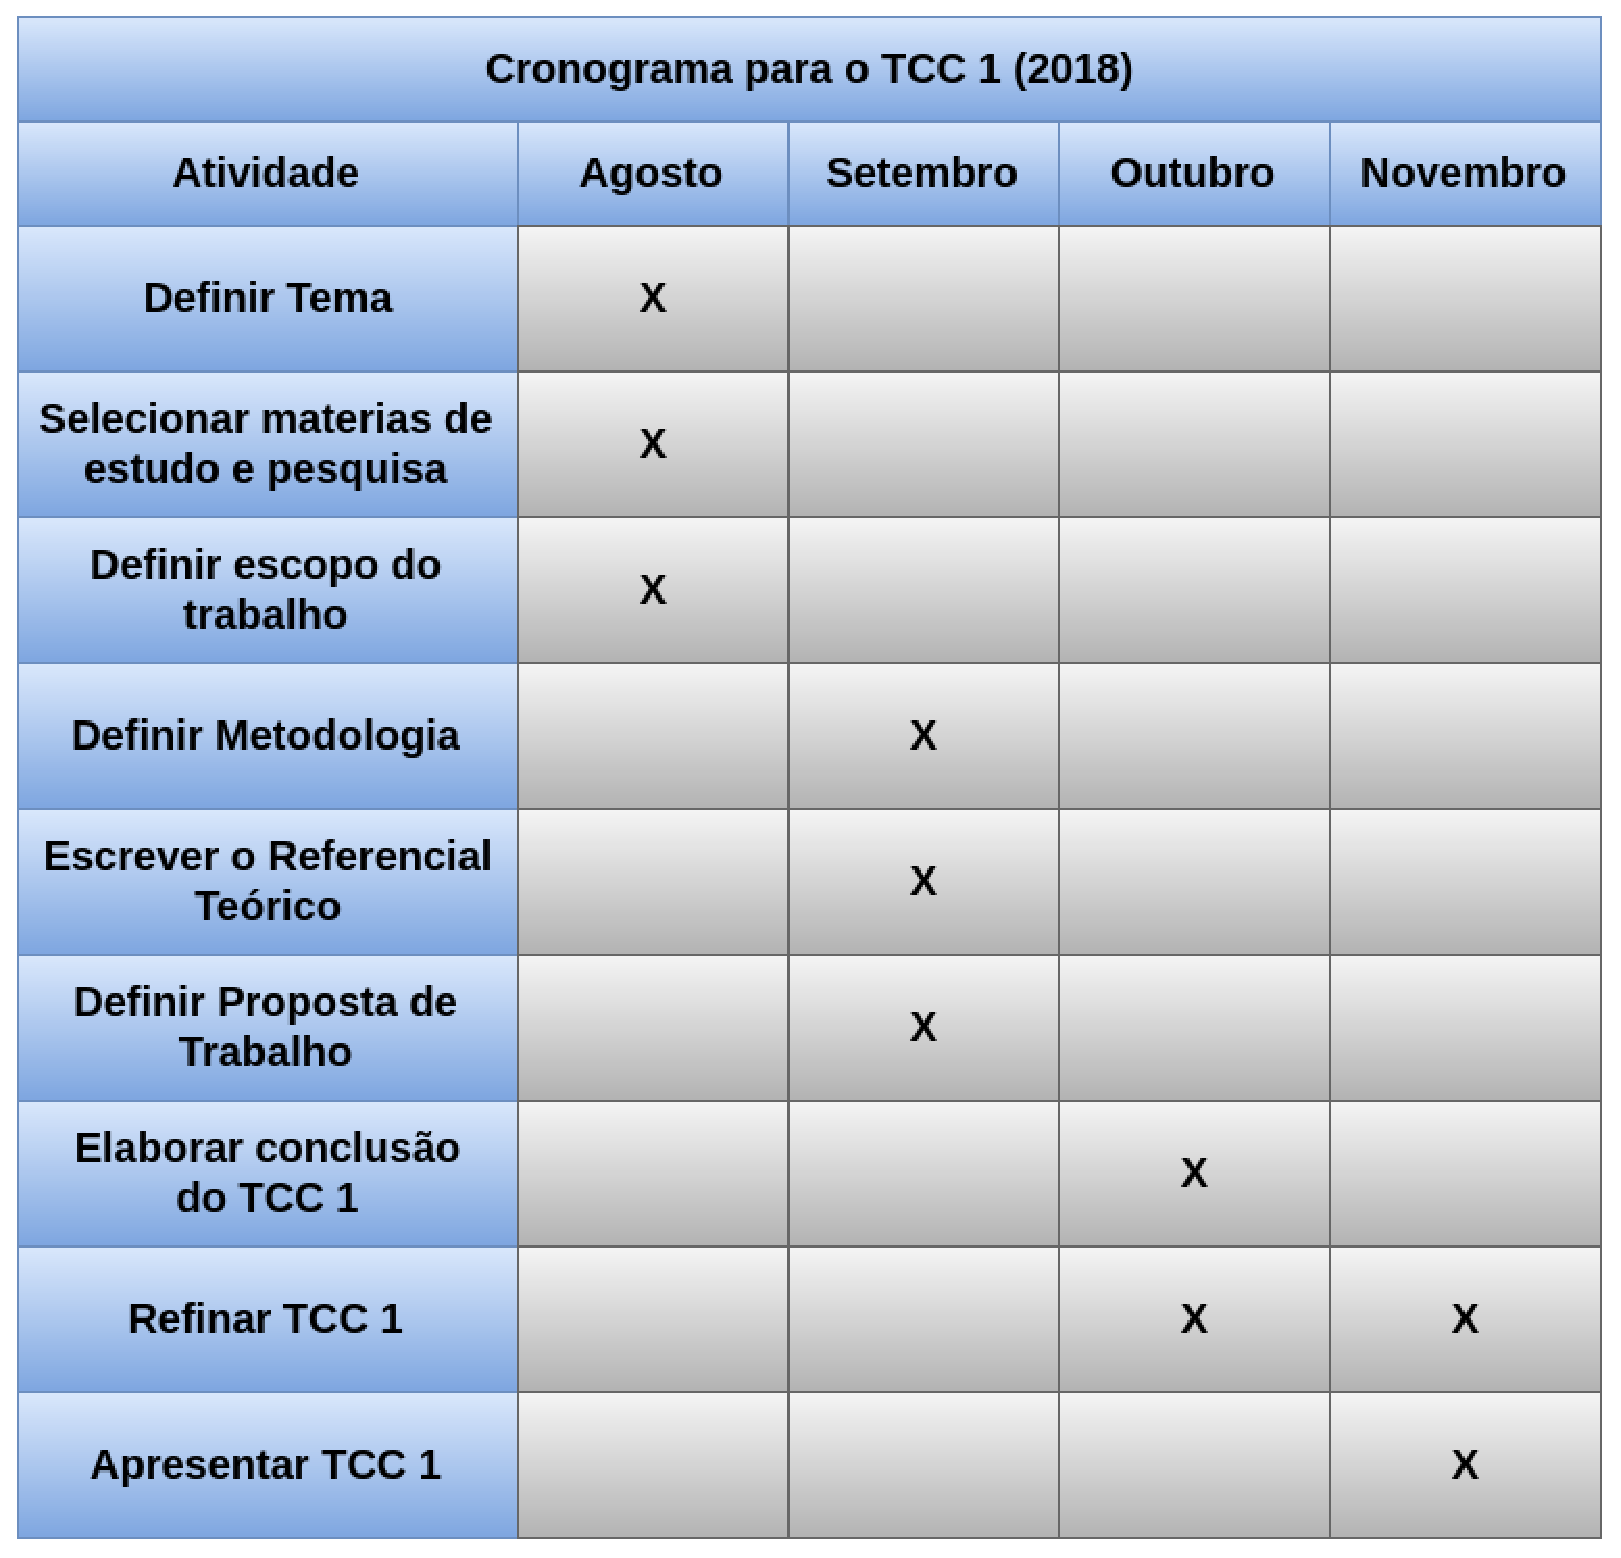
\includegraphics[keepaspectratio=true,scale=0.4]{figuras/cronograma_tcc1.eps}
  \caption[Cronograma do TCC 1.]{Cronograma do TCC 1. Fonte: Autor}
	\label{fig:cronograma_tcc1}
\end{figure}

\subsection{Marco 2: Trabalho de Conclusão de Curso 2}

Dando entrada no marco 2 do projeto será feito os ajustes necessários do TCC 1 para o trabalho de conclusão de curso 2 ou TCC 2. Com isso será documentado de forma sucinta os resultados da metodologia aplicada no processo de desenvolvimento. E em paralelo será documentado os resultados do software e sua aplicação em um contexto real.

Assim que os resultados estiverem documentados será elaborado a conclusão do TCC 2 e será feito uma verificação geral no documento para melhorá-lo. Com o trabalho pronto, será criado os slides da apresentação do TCC 2 e assim finalizar o marco 2 do projeto.

Em concordância com o processo de condução do TCC2 foi elaborado o cronograma da figura \ref{fig:cronograma_tcc2}:

\begin{figure}[h!]
	\centering
  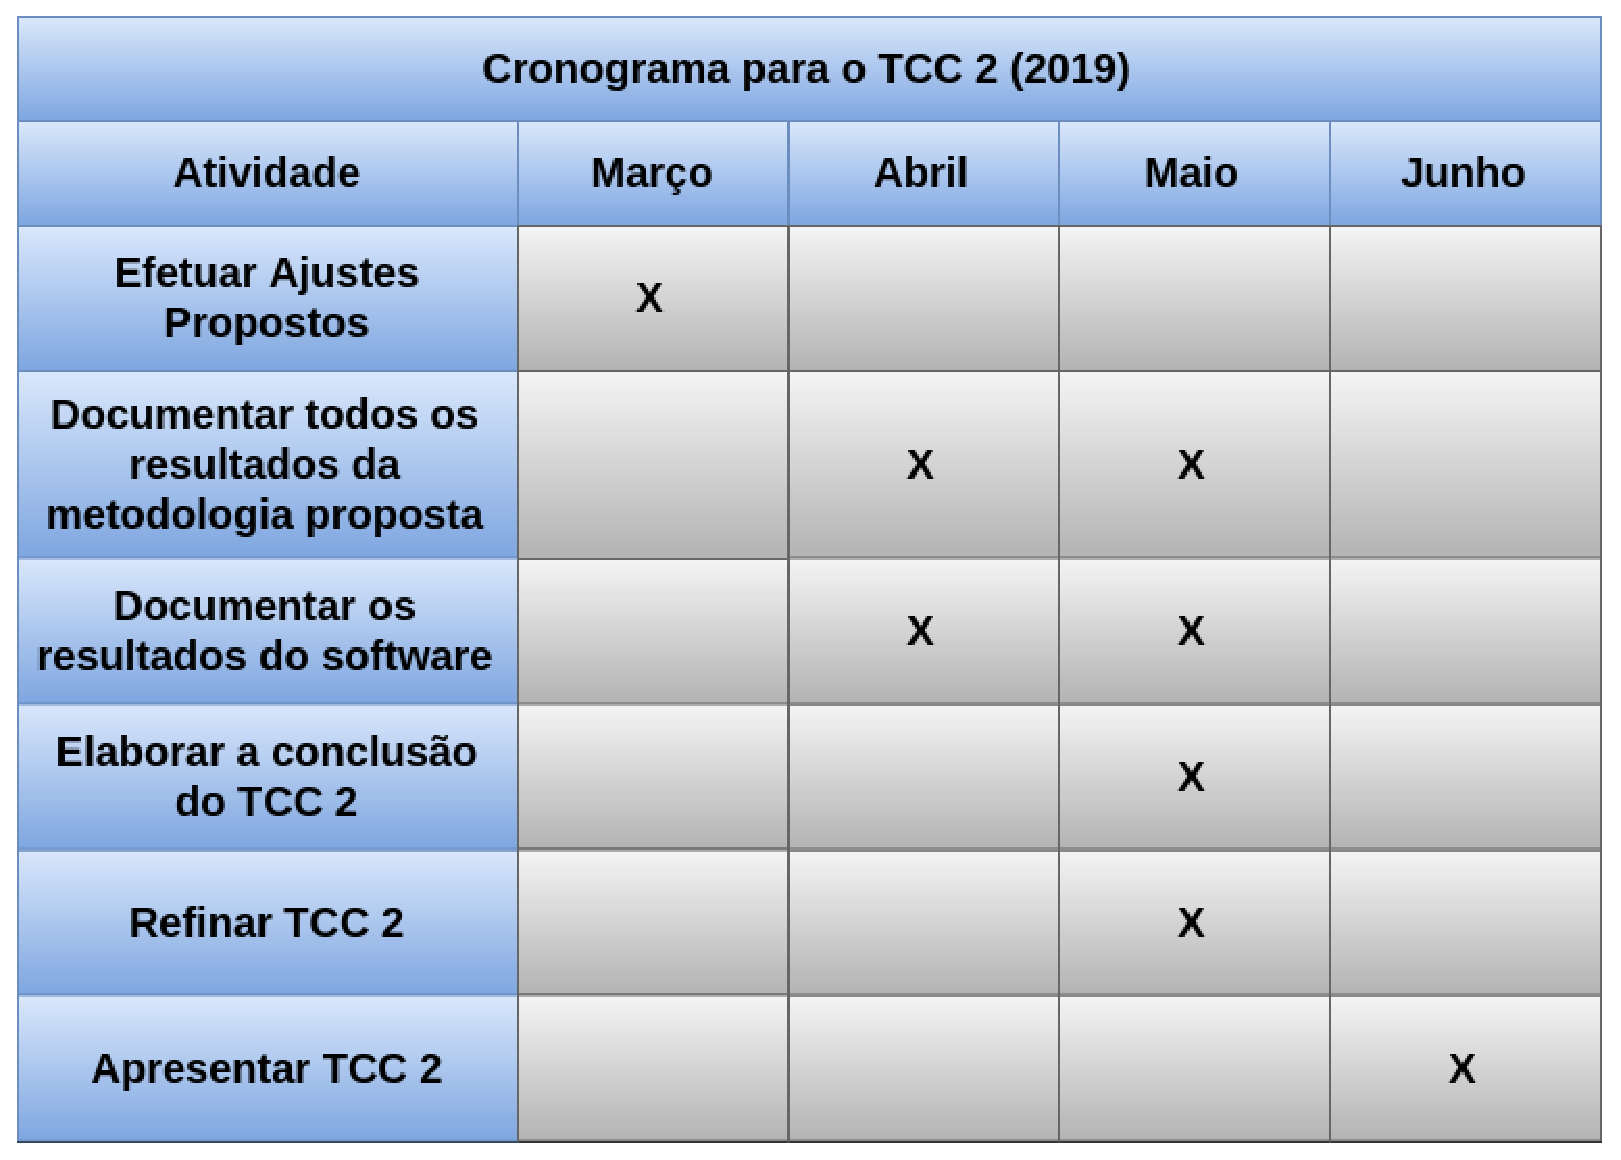
\includegraphics[keepaspectratio=true,scale=0.4]{figuras/cronograma_tcc2.eps}
  \caption[Cronograma do TCC 2.]{Cronograma do TCC 2. Fonte: Autor}
	\label{fig:cronograma_tcc2}
\end{figure}
